\documentclass[12pt,a4paper]{article}
\usepackage{amsmath,amssymb}
\usepackage{graphicx}
\usepackage{float}
\usepackage{tikz}
\usetikzlibrary{shapes, arrows, positioning}


\usepackage{amsmath,amssymb,mdframed}            % AMS package gives better equation layouts
\setcounter{page}{5}                    % sets first page number to 2
\setlength{\oddsidemargin}{-0.25in}     % set left margin
\setlength{\textwidth}{6.5in}           % set text width
\setlength{\topmargin}{-0.5in}          % controls layout at
\setlength{\headsep}{0.5in}             % top of page
\setlength{\textheight}{9.0in}          % set text length



\makeatletter
\renewcommand{\@oddhead}{\hfill MA3600/2014-2015-resit-solution}  % sets header
\renewcommand{\@oddfoot}{\hfil \arabic{page} \hfil}    % sets page footer
\makeatother

\renewcommand{\labelenumi}{\arabic{enumi}} % Sets the first level of enumerate to be arabic (normal) numbers
\renewcommand{\labelenumii}{(\alph{enumii})} %Sets the second level of enumerate to be (a), (b), (c), .....
\renewcommand{\labelenumiii}{(\roman{enumiii})} % Sets the third level of enumerate to be (i), (ii), (iii), ....



\begin{document}
\null \vskip1cm
\begin{enumerate}
\setcounter{enumi}{3}

\renewcommand\labelenumi{\bfseries\theenumi.}

\item

    \begin{enumerate}
        \item Provide definitions for the following terms:
            \begin{itemize}
                \item Normal form game.\\


                A $N$ player \textbf{normal form game} consists of:
                \begin{itemize}
                \item A finite set of $N$ players;
                \item Strategy spaces for the players: $S_1, S_2, S_3, \dots S_N$;
                \item Payoff functions for the players: $u_i:S_{1}\times S_2\dots\times S_N\to \mathbb{R}$
                \end{itemize}

                ~\hfill{[1]}

                \item Strictly dominated strategy.\\

                In an $N$ player normal form game. A pure strategy $s_i\in S_i$ is said to be \textbf{strictly dominated} if there is a strategy $\sigma_i\in \Delta S_i$ such that $u_i(\sigma_i,s_{-i})>u_{i}(s_i,s_{-i})$ for all $s_{-i}\in S_{-i}$ of the other players.

                ~\hfill{[1]}

                \item Weakly dominated strategy.\\

                In an $N$ player normal form game. A pure strategy $s_i\in S_i$ is said to be \textbf{weakly dominated} if there is a strategy $\sigma_i\in \Delta S_i$ such that $u_i(\sigma_i,s_{-i})\geq u_{i}(s_i,s_{-i})$ for all $s_{-i}\in S_{-i}$ of the other players and there exists a strategy profile $\bar s\in S_{-i}$ such that $u_i(\sigma_i,\bar s)> u_{i}(s_i,s_{-i})$.

                ~\hfill{[1]}

                \item Best response strategy.\\

                In an $N$ player normal form game. A strategy $s^*$ for player $i$ is a best response to some strategy profile $s_{-i}$ if and only if $u_i(s^*,s_{-i})\geq u_{i}(s,s_{-i})$ for all $s\in S_i$.

                ~\hfill{[1]}

                \item Nash equilibrium.\\

                In an $N$ player normal form game. A Nash equilibrium is a strategy profile $\tau = (\tilde s_1,\tilde s_2,\dots,\tilde s_N)$ such that:

                $$u_i(\tilde s)\geq u_i(\bar s_i,\tilde s_{-i})\text{ for all }i$$
                ~\hfill{[1]}
            \end{itemize}

        \item     Consider the following game:

            \[\begin{pmatrix}
            (1,\alpha) & (0,2)\\
            (0,0) & (\alpha,1)\\
            \end{pmatrix}\]

            \begin{enumerate}
            \item Prove that a pure Nash equilibrium exists for all values of
                \(\alpha \in \mathbb{R}\).

                If \(\alpha\leq 0\) then the best responses are given by:

                    \[\begin{pmatrix}
                        (\underline{1},\alpha) & (\underline{0},\underline{2})\\
                        (0,0) & (\alpha,\underline{1})\\
                    \end{pmatrix}\]

                So \((r_1, c_2)\) is a pure Nash equilibrium.

            ~\hfill{[2]}

                If \(2\geq\alpha\geq 0\) then the best responses are given by:

                    \[\begin{pmatrix}
                        (\underline{1},\alpha) & (0,\underline{2})\\
                        (0,0) & (\underline{\alpha},\underline{1})\\
                    \end{pmatrix}\]

                So \((r_2, c_2)\) is a pure Nash equilibrium.

            ~\hfill{[2]}

                If \(2\leq\alpha\) then the best responses are given by:

                    \[\begin{pmatrix}
                        (\underline{1},\underline{\alpha}) & (0,2)\\
                        (0,0) & (\underline{\alpha},\underline{1})\\
                    \end{pmatrix}\]

                So \((r_1, c_1)\) and \((r_2, c_2)\) are pure Nash equilibrium.

            ~\hfill{[3]}

            \item State the equality of payoffs theorem. Using this theorem
                obtain the value of \(\alpha\) (if it exists) for which the
                following \((\sigma_1, \sigma_2)\) are mixed Nash equilibria for the game.

            The equality of payoffs theorem states:

            In an $N$ player normal form game if the strategy profile $(\sigma_i,s_{-i})$ is a Nash equilibria then:

            $$u_{i}(\sigma_i,s_{-i})=u_{i}(s,s_{-i})\text{ for all }s\in\mathcal{S}(\sigma_i)\text{ for all }1\leq i\leq N$$

            ~\hfill{[1]}

                \begin{enumerate}
                    \item \((\sigma_1, \sigma_2) = ((1/2,1/2), (1/2,1/2))\)

                    If \(((1/2,1/2), (1/2,1/2))\) is a Nash equilibrium the
                    equality of payoffs theorem states:

                    \[u_2((1/2,1/2),c_1)=u_2((1/2,1/2),c_2)\]

                    which implies:

                    \[\alpha/2=3/2\]

                    ~\hfill{[2]}

                    So \(\alpha=3\). If \(\alpha=3\) then

                    \[u_1(r_1, (1/2,1/2))=1/2\quad u_1(r_2, (1/2,1/2))=3/2\]

                    Thus by the equality of payoffs theorem this is not a Nash
                    equilibrium.

                    ~\hfill{[2]}

                    \item \((\sigma_1, \sigma_2) = ((1/2,1/2), (3/4,1/4))\)

                    If \(((1/2,1/2), (3/4,1/4))\) is a Nash equilibrium the
                    equality of payoffs theorem states:

                    \[u_2((1/2,1/2),c_1)=u_2((1/2,1/2),c_2)\]

                    which implies:

                    \[\alpha/2=3/2\]

                    ~\hfill{[2]}

                    So \(\alpha=3\). If \(\alpha=3\) then

                    \[u_1(r_1, (3/4,1/4))=3/4\quad u_1(r_2, (3/4,1/4))=3/4\]

                    Thus by the equality of payoffs theorem this is a Nash
                    equilibrium.

                    ~\hfill{[2]}

                    \item \((\sigma_1, \sigma_2) = ((1/5,4/5), (3/4,1/4))\)

                    If \(((1/5,4/5), (3/4,1/4))\) is a Nash equilibrium the
                    equality of payoffs theorem states:

                    \[u_2((1/5,4/5),c_1)=u_2((1/5,4/5),c_2)\]

                    which implies:

                    \[\alpha/5=6/5\]

                    ~\hfill{[2]}

                    So \(\alpha=6\). If \(\alpha=6\) then

                    \[u_1(r_1, (1/4,3/4))=1/4\quad u_1(r_2, (1/4,3/4))=3\times6/4\]

                    Thus by the equality of payoffs theorem this is not a Nash
                    equilibrium.

                    ~\hfill{[2]}
                \end{enumerate}


            \end{enumerate}


    \end{enumerate}

\newpage
\item

    \begin{enumerate}
        \item Define a (finitely) repeated game.

            A repeated game is played over discrete time periods. Each time
            period is index by \(0<t\leq T\) where \(T\) is the total number of
            periods.  In each period \(N\) players play a static game referred
            to as the \textbf{stage game} independently and simultaneously
            selecting actions.  Players make decisions in full knowledge of the
            \textbf{history} of the game played so far (ie the actions chosen by
            each player in each previous time period).  The payoff is defined as
            the sum of the utilities in each stage game for every time period.

        ~\hfill[4]

        \item Define a strategy in a repeated game.

            A repeated game strategy must specify the action of a player in a given stage
            game given the entire history of the repeated game.

        ~\hfill[2]

        \item Prove that for any repeated game, any sequence of stage Nash profiles
            gives the outcome of a subgame perfect Nash equilibrium.

            If we consider the strategy given by:

            "Player \(i\) should play strategy \(\tilde s^{(k)}_i\) regardless of the play
            of any previous strategy profiles."

        ~\hfill[3]

            where \(\tilde s^{(k)}_i\) is the strategy played by player \(i\) in any stage
            Nash profile. The \(k\) is used to indicate that all players play strategies
            from the same stage Nash profile.

            Using backwards induction we see that this strategy is a Nash equilibrium.

        ~\hfill[2]

            Furthermore it is a stage Nash profile so it is a Nash equilibria for the last
            stage game which is the last subgame. If we consider (in an inductive way) each
            subsequent subgame the result holds.

        ~\hfill[2]

        \item For the following stage games, plot the possible outcomes for a
            repetition of \(T=2\) periods and obtain a Nash equilibria
            \textbf{that is not a sequence of stage Nash profiles}:

            \[
                \begin{pmatrix}
                    (3,4) & (1,2) & (2,5)\\
                    (-1,1) & (1,2) & (-1,-1)
                \end{pmatrix}
            \]

            Here is the plot:

            \begin{center}
                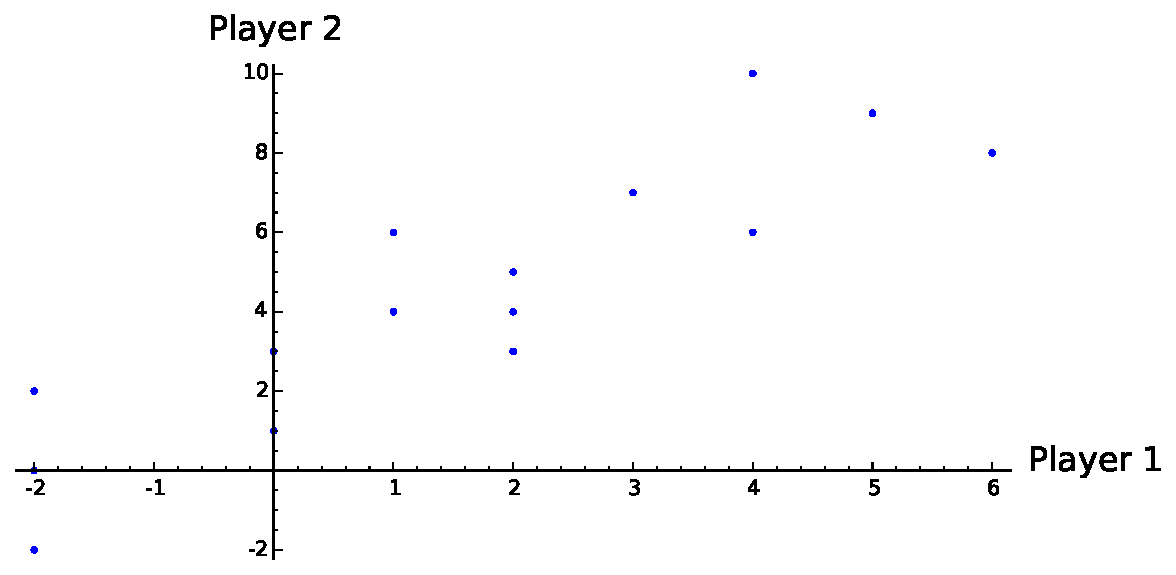
\includegraphics[width=.6\textwidth]{plots/resit-sol-2013-2014-plt01.pdf}
            \end{center}

            ~\hfill[1]

            The following is a subgame perfect NE: play \((r_1, c_1)\) in first
            round and \((r_1, c_3)\) in second round. If not, play \((r_2, c_2)\) in
            second.

            ~\hfill[1]

            This is subgame perfect:

            \begin{itemize}
                \item First player has no incentive to deviate;
                \item Second player can deviate in first to gain 1, but will
                    lose 3 in second round.
                \item First subgame: playing stage NE.
            \end{itemize}

            ~\hfill[1]

            \[
                \begin{pmatrix}
                    (3,1) & (1,1)\\
                    (-1,1) & (1,0)\\
                    (1,3) & (.5,1)\\
                \end{pmatrix}
            \]

            Here is the plot:

            \begin{center}
                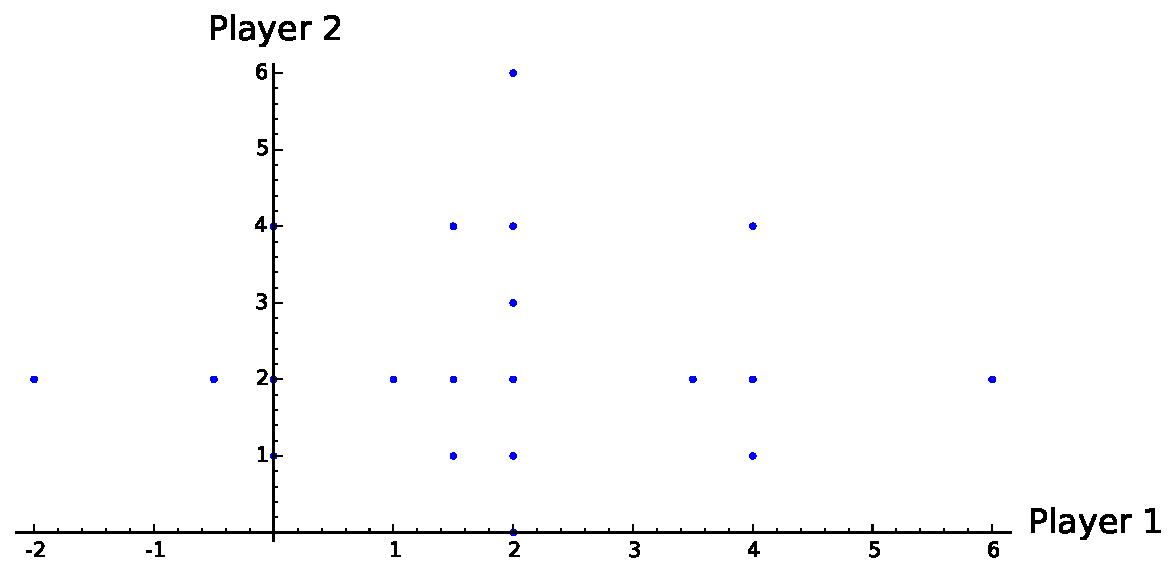
\includegraphics[width=.6\textwidth]{plots/resit-sol-2013-2014-plt02.pdf}
            \end{center}

            ~\hfill[1]

            The following is a subgame perfect NE: play \((r_3, c_1)\) in first
            round and \((r_1, c_1)\) in second round. If not, play \((r_1, c_2)\) in second.

            ~\hfill[1]

            This is subgame perfect:

            \begin{itemize}
                \item Second player has no incentive to deviate;
                \item First player can deviate in first to gain 2, but will
                    lose 2 in second round so no incentive.
                \item First subgame: playing stage NE.
            \end{itemize}

            ~\hfill[1]

            \[
                \begin{pmatrix}
                    (2,9) & (3,1)\\
                    (3,1) & (6,1)\\
                    (3,3) & (5,1)\\
                \end{pmatrix}
            \]

            Here is the plot:

            \begin{center}
                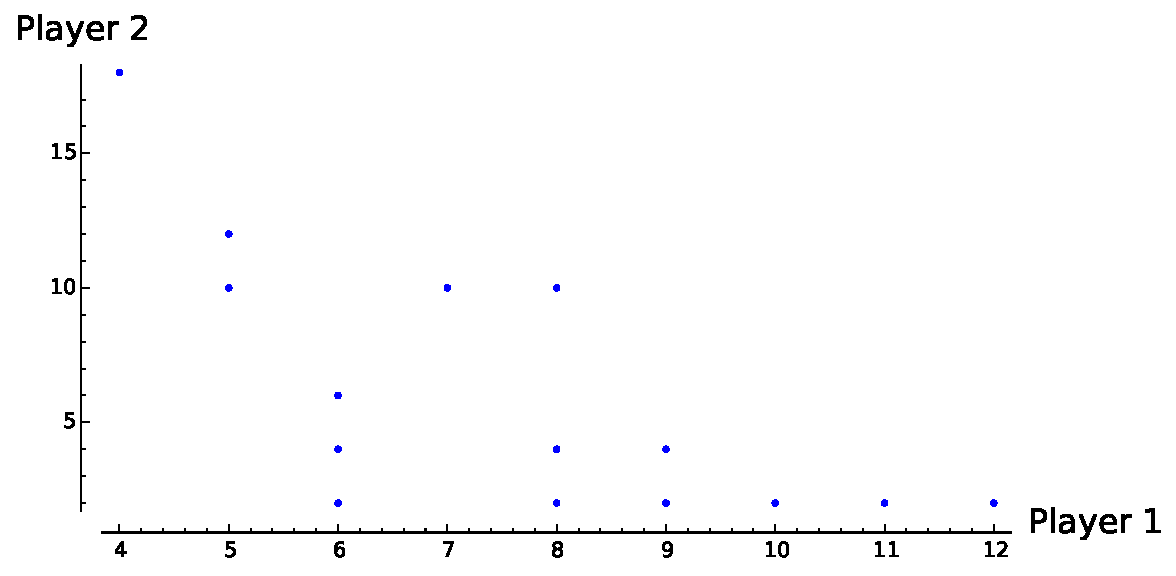
\includegraphics[width=.6\textwidth]{plots/resit-sol-2013-2014-plt03.pdf}
            \end{center}

            ~\hfill[1]

            The following is a subgame perfect NE: play \((r_1, c_1)\) in first
            round and \((r_2, c_2)\) in second round. If not, play \((r_3, c_1)\) in second.

            ~\hfill[1]

            This is subgame perfect:

            \begin{itemize}
                \item Second player has no incentive to deviate;
                \item First player can deviate in first to gain 1, but will
                    lose 3 in second round so no incentive.
                \item First subgame: playing stage NE.
            \end{itemize}

            ~\hfill[1]

            \[
                \begin{pmatrix}
                    (1,1) & (1,0) & (1,1)\\
                    (1,2) & (3,2) & (2,5)
                \end{pmatrix}
            \]

            Here is the plot:

            \begin{center}
                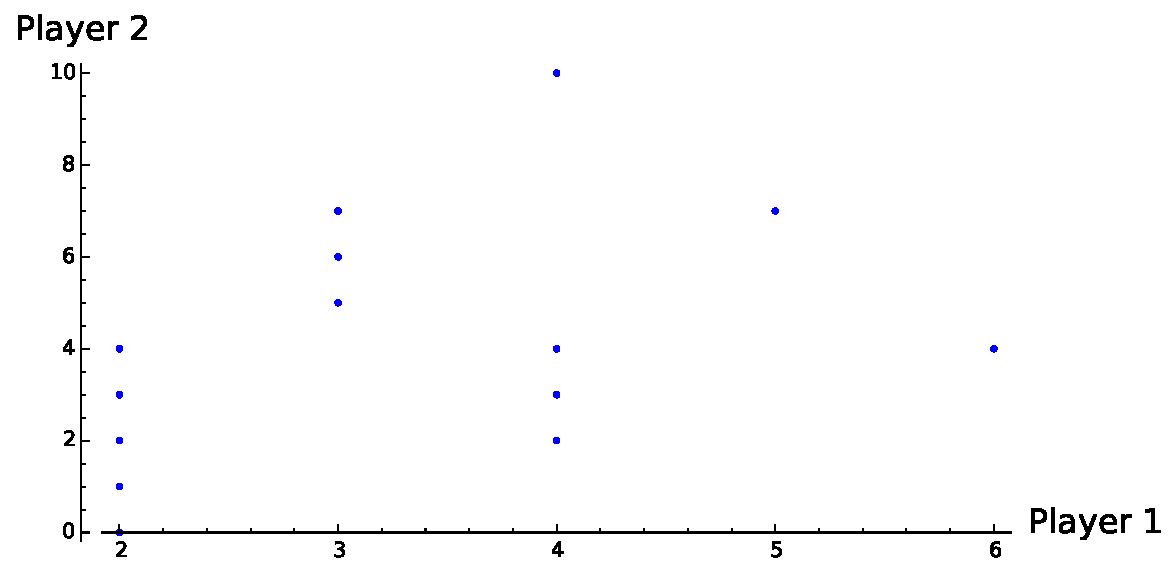
\includegraphics[width=.6\textwidth]{plots/resit-sol-2013-2014-plt04.pdf}
            \end{center}

            ~\hfill[1]

            The following is a subgame perfect NE: play \((r_2, c_2)\) in first
            round and \((r_2, c_3)\) in second round. If not, play \((r_1, c_1)\) in second.

            ~\hfill[1]

            This is subgame perfect:

            \begin{itemize}
                \item First player has no incentive to deviate;
                \item Second player can deviate in first to gain 3, but will
                    lose 4 in second round so no incentive.
                \item First subgame: playing stage NE.
            \end{itemize}

            ~\hfill[1]

    \end{enumerate}

\newpage
\item

    \begin{enumerate}

        \item Define a stochastic game.

        A stochastic game is defined by:

        \begin{itemize}
            \item X a set of states with a stage game defined for each state;
            \item A set of strategies \(S_i(x)\) for each player for each state \(x\in X\);
            \item A set of rewards dependant on the state and the actions of the other players: \(u_i(x,s_1,s_2)\);
            \item A set of probabilities of transitioning to a future state: \(\pi(x'\|x,s_1,s_2)\);
            \item Each stage game is played at a set of discrete times \(t\).
        \end{itemize}

        \hfill[4]

        \item Define a Markov strategy.

        A strategy is call a \textbf{Markov strategy} if the behaviour dictated is not time dependent.

        \hfill[2]

        \item Give the conditions for Nash equilibrium in a stochastic game.

            A Nash equilibrium satisfies:

            $$U_1^*(x)=\max_{r\in S_1(x)}(u_i(x,r,s^*)+\delta\sum_{x'\in X}\pi(x'|x,r,s^*)U_1^*(x')$$
            $$U_2^*(x)=\max_{s\in S_2(x)}(u_i(x,r^*,s)+\delta\sum_{x'\in X}\pi(x'|x,r^*,s)U_1^*(x')$$

        \hfill[3]

        \item Obtain the pure strategy Nash equilibria (if any exist) for the
            following game with \(\delta=.3\):

        \begin{center}
            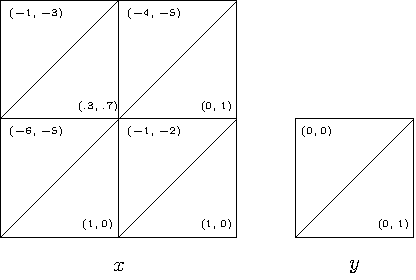
\includegraphics[width=.8\textwidth]{images/2014-2015-resit-img01.pdf}
        \end{center}

        State \(y\) gives no value to either player so we only need to consider state \(x\). Let the future gains to 1 in state \(x\) by \(u\) and the future gains to player 2 in state \(x\) be \(v\). Thus the players are facing the following game:

        \hfill[2]

        \[\begin{pmatrix}
        (-1+9/100u,-3+9/100v)&(-4,-5)\\
        (-6+3/10u,-5+3/10v)&(-1+3/10u,-2+3/10v)
        \end{pmatrix}\]

        \hfill[2]

        There are 4 potential pure strategy equilibrium:

        \begin{itemize}
            \item \((a,c)\) which requires \(-1+9/100u\geq -6+3/10u\) and
                \(-3+9/100v\geq -5\) \(\Rightarrow\) \(u\leq 500/21\) and
                \(v\geq -200/9\). If this is the equilibria then \(u=-1+9/100u\)
                which gives \(u=-100/91\) and \(-3+9/100v=v\) which gives
                \(v=-300/91\). This contradicts no constraints.

                ~\hfill[3]

            \item \((a,d)\) which requires \(-4\geq -1+3/10u\) and
                \(-3+9/100v\leq -5\) \(\Rightarrow\) \(u\leq -10\) and
                \(v\leq -200/9\). If this is the equilibria then \(u=-4\)
                which gives \(u=-5\). This contradicts both constraints.

                ~\hfill[3]

            \item \((b,c)\) which requires \(-1+9/100u\leq -6+3/10u\) and
                \(-5+3/10v\geq -2+3/10v\), this later inequality has no
                solution.

                ~\hfill[3]

            \item \((b,d)\) which requires \(-4\leq -1+3/10u\) and
                \(-5+3/10v\leq -2+3/10v\)) \(\Rightarrow\) \(u\geq -10\) and
                \(v \in \mathbb{R}\). If this is the equilibria then \(u=-1+3/10u\)
                which gives \(u=-10/7\) and \(-2+3/10v=v\) which gives
                \(v=-20/7\). This contradicts no constraints.

                ~\hfill[3]
        \end{itemize}

        Thus \((a,c)\) and \((b,d)\) are the Nash Equilibria for this stochastic
        game.

    \end{enumerate}
\end{enumerate}


\makeatletter
\renewcommand{\@oddfoot}{\hfil \arabic{page}X \hfil}    % sets last page footer
\makeatother

\end{document}
